\chapter{Top-down maze resolution approach}

\section{Background}

This task was developed in python. The imports used are listed below.

\begin{itemize}
\item The following libraries were used in maze\_generator:
\begin{itemize}
\item \lstinline {from queue import LifoQueue }: it is used to create a Last In First Out stack where adjacent nodes are inserted.

\item \lstinline{from PIL import Image}: 
it is used to create images where mazes are saved graphically.
\item  \lstinline{import numpy as np}: 
creates cells and fills them with zero. It is used to initialize the maze.
\item  \lstinline{from random import choice}: 
it is used to randomly choose a neighbor so that the mazes are always all different.
\item  \lstinline{import agents}: 
sets up agents in the maze

\item  \lstinline{import argparse}: makes it easy to write intuitive command line interfaces. The argparse module is useful because it also automatically generates help and usage messages and generates errors when users provide invalid arguments to the program.
\item  \lstinline{ import os}: it is used to create the folder containing the mazes.
\item  \lstinline{ import sys}: 
it is used to do multiple runs of the same code.
\end{itemize}

\item The following libraries were used in agents:
\begin{itemize}


\item \lstinline {import cv2 }: 
it is used to read the maze image and add agents to it.
\item \lstinline{import random}: it is used to place the red agent in a random position in path.
\item  \lstinline{import numpy as np}: it is used to find all valid positions in the maze.

\end{itemize}
\item The following libraries were used in maze\_analyser:
\begin{itemize}
\item \lstinline {from typing import List }: generates a list of nodes for a maze for navigation so that they are linked up width weighted edges based on the distance from one another in the maze.
\end{itemize}
\item The following libraries were used in dijkstra:
\begin{itemize}

\item \lstinline{import functools}: 
serves for higher-order functions: functions that act or return other functions.
\item  \lstinline{from queue import PriorityQueue}: 
it is used to keep in memory the stack of nodes that make up the path between the start node and the finish node
\item  \lstinline{from typing import List}: 
it is used to return the list of nodes that form the shortest path to reach the agent.

\item \lstinline{import numpy as np}: used to create color fades between blue and red (only used to improve the readability of the solution).
\item  \lstinline{from PIL import Image}: 
used to open the maze image (input image) and to load its pixels. Finally used to save the new output image.
\item  \lstinline{import time}: used to calculate the execution time of the Dijkstra algorithm
\item  \lstinline{import os}: 
used to create the results folder and save the images that solve the mazes in it.

\item  \lstinline{from maze_analyser import Node, nodes_from_maze}: 
used as an input to the algorithm. To know how the maze is made and then subsequently be able to solve it.
\item  \lstinline{  import argparse}: 
Used in the same way as maze\_analyser.
\end{itemize}
\end{itemize}
\section{Implementation}

For this type of task we need 4 files. To show how it works, run \textit{maze\_generator.py} and then \textit{dijkstra.py}: 2 folders will appear, one with the generated mazes and one with the resolution of these. 
\begin{itemize}
\item \textbf{maze\_generator}: creates the mazes with different sizes. With the settings currently set, it creates 10 mazes with 3 different sizes. The mazes consist of a white path, black walls and two agents. The blue agent is always positioned at the entrance to the maze in the coordinates (1,0) while the red agent is positioned randomly. The output is saved in an image
\item\textbf{agents }: creates the agents and place them in the maze. 
\item\textbf{maze\_analyser}: analyzes the image of the maze, keeps in memory the position of the blue agent (start position), all the nodes on which it could move (the path) and the position of the red agent (the arrival position).  The maze must be made up of black and white pixels, the start point must be either on the left and top side,the end point must be on the red agent.
	
\item \textbf{dijkstra}: Using the input values ​​provided by maze \_analyser it searches for the shortest path from the initial node (blue agent) to the final node (red agent). Dijkstra's algorithm is used to find the shortest path. Once the set of nodes forming the shortest path is found, this path is saved to an image and colored in a blue to red gradient. Finally, the blue agent is placed in place of the red agent to simulate its displacement.
\end{itemize}

\textbf{Dijkstra's algorithm} is an algorithm for finding the shortest paths between nodes in a graph. It is uses labels that are positive integers numbers, which are totally ordered.
Dijkstra's algorithm uses a data structure for storing and querying partial solutions sorted by distance from the start.
Let the node at which we are starting be called the initial node (in our case the blue agent). Let the distance of node Y be the distance from the initial node to Y. 
The final node will be the red agent who is randomly placed in the maze (in the white path).
Dijkstra's algorithm will assign some initial distance values and will try to improve them step by step. 


\begin{figure}[h]
\centering
\begin{minipage}{.5\textwidth}
\centering
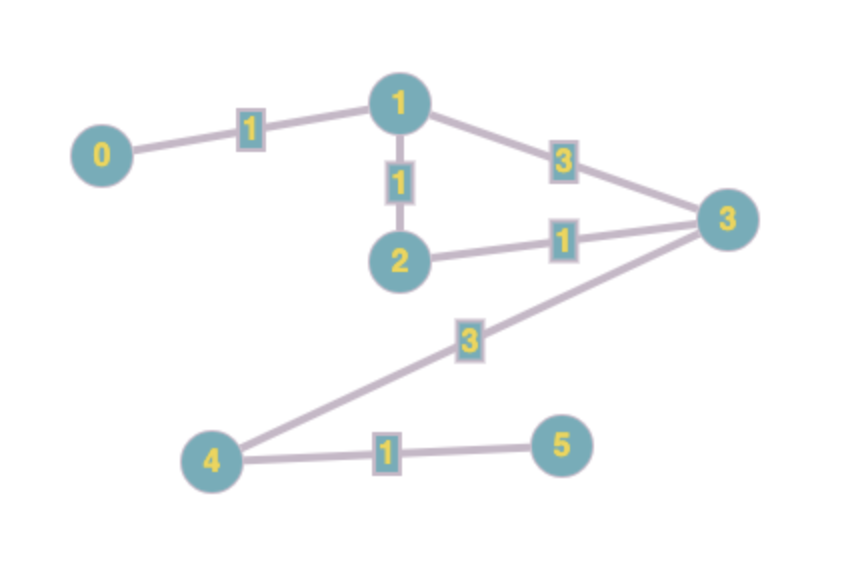
\includegraphics[width=0.7\linewidth]{img/dijkstraex}
  \caption{Dijkstra example}
  \label{fig:dijkstraex}
\end{minipage}%
\begin{minipage}{.5\textwidth}
\centering
	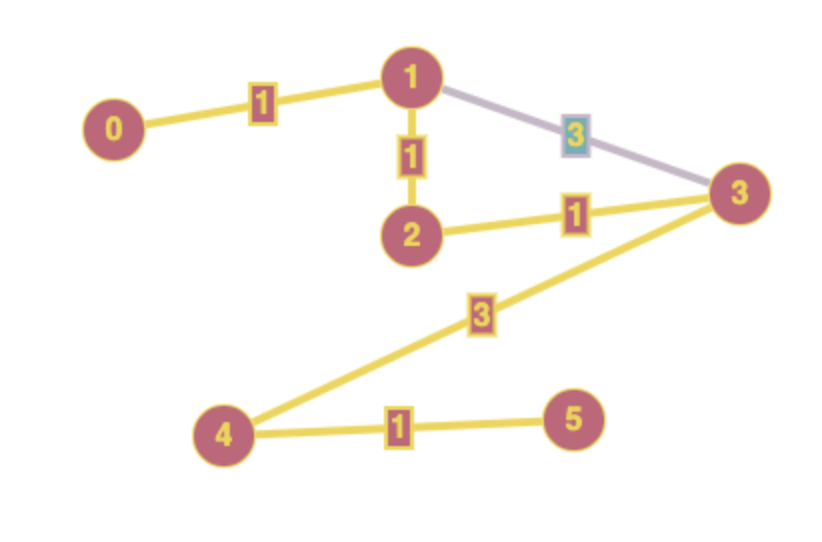
\includegraphics[width=0.7\linewidth]{img/dijkexsolved}
	\caption{Dijkstra example solved}
	\label{fig:dijkexsolved}
\end{minipage}

\end{figure}


\begin{figure}[h]
\centering
\begin{minipage}{.3\textwidth}
\centering
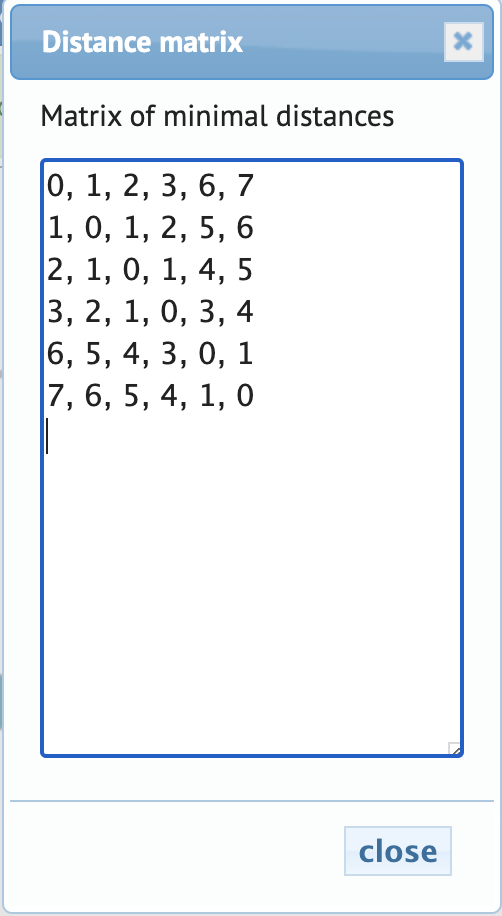
\includegraphics[width=0.65\linewidth]{img/DistanceMatrix}

\end{minipage}%
\begin{minipage}{.3\textwidth}
\centering
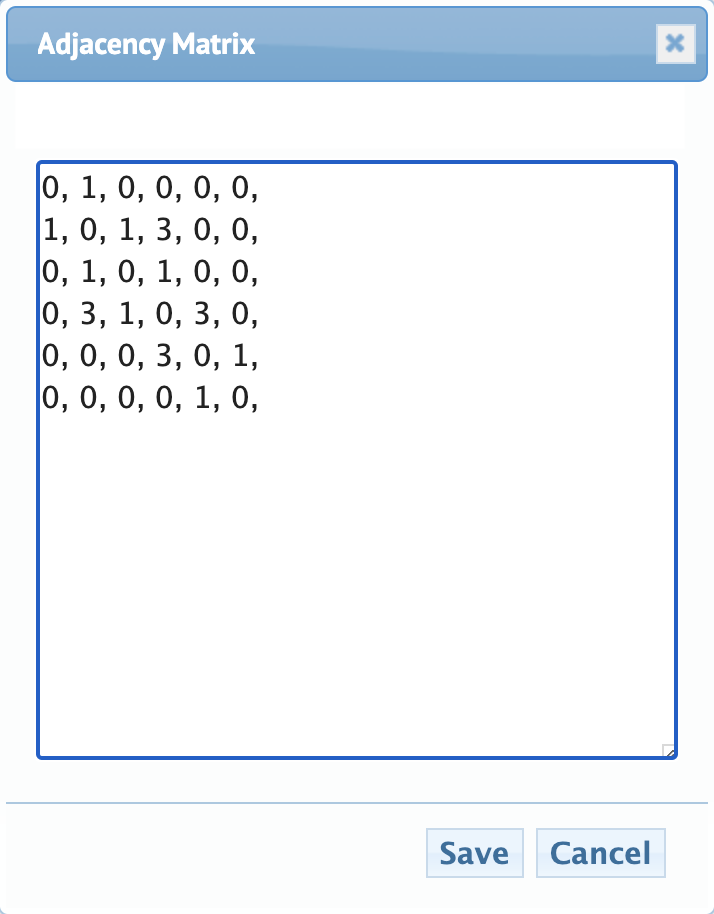
\includegraphics[width=0.85\linewidth]{img/AdjacencyMatrix}

\end{minipage}

\begin{minipage}{.3\textwidth}
\centering
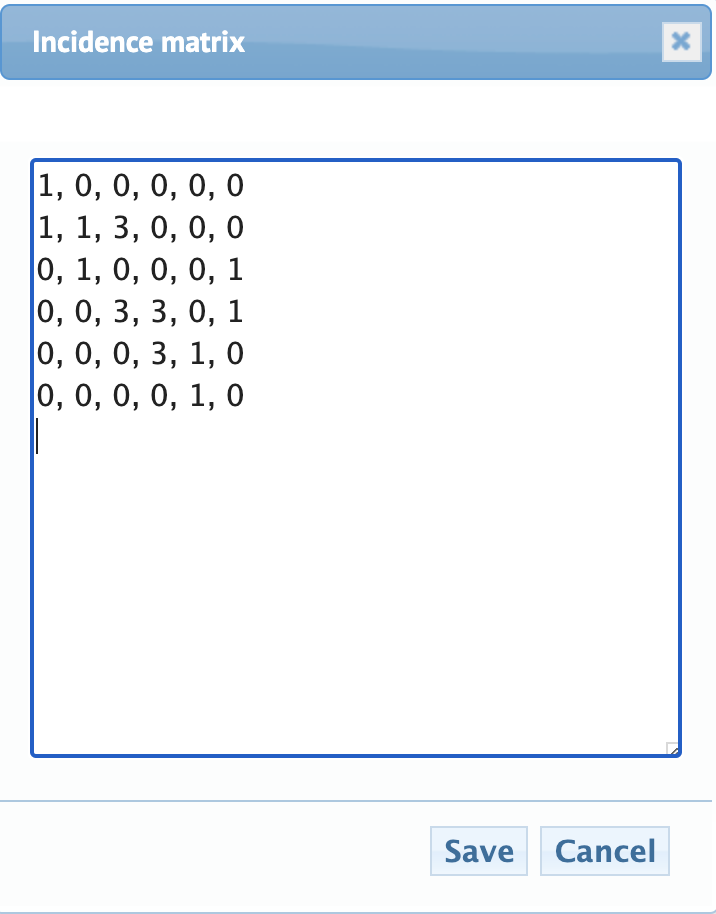
\includegraphics[width=0.85\linewidth]{img/IncidenceMatrix}
\caption{Distance Matrix, Adjacency Matrix and Incidence Matrix}
\label{fig:incidencematrix}
\end{minipage}
\end{figure}


\subsection{Output}
The resulting output will be the fastest path from agent blue to agent red. For example, from the situation on the left (Figure \ref{fig:maze}) generated with maze\_generator, Dijkstra's algorithm will produce the solution on the right (Figure \ref{fig:mazesolved}). This maze is one of the simplest generated but the difficulty can be increased by setting the file maze\_generator. All mazes have a solution and the red agent does not move since Dijkstra's algorithm does not learn so it would never be able to reach the red agent if it moved.
\begin{figure}[h]
\centering
\begin{minipage}{.5\textwidth}
\centering
 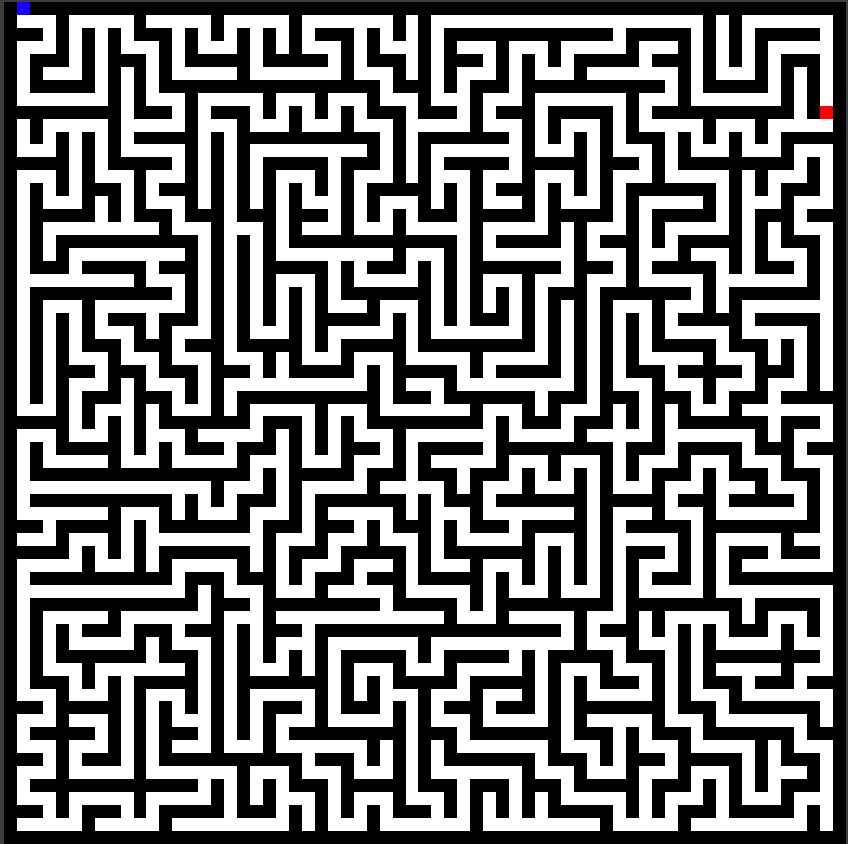
\includegraphics[width=0.8\linewidth]{img/maze}
  \caption{Maze}
  \label{fig:maze}
\end{minipage}%
\begin{minipage}{.5\textwidth}
\centering
	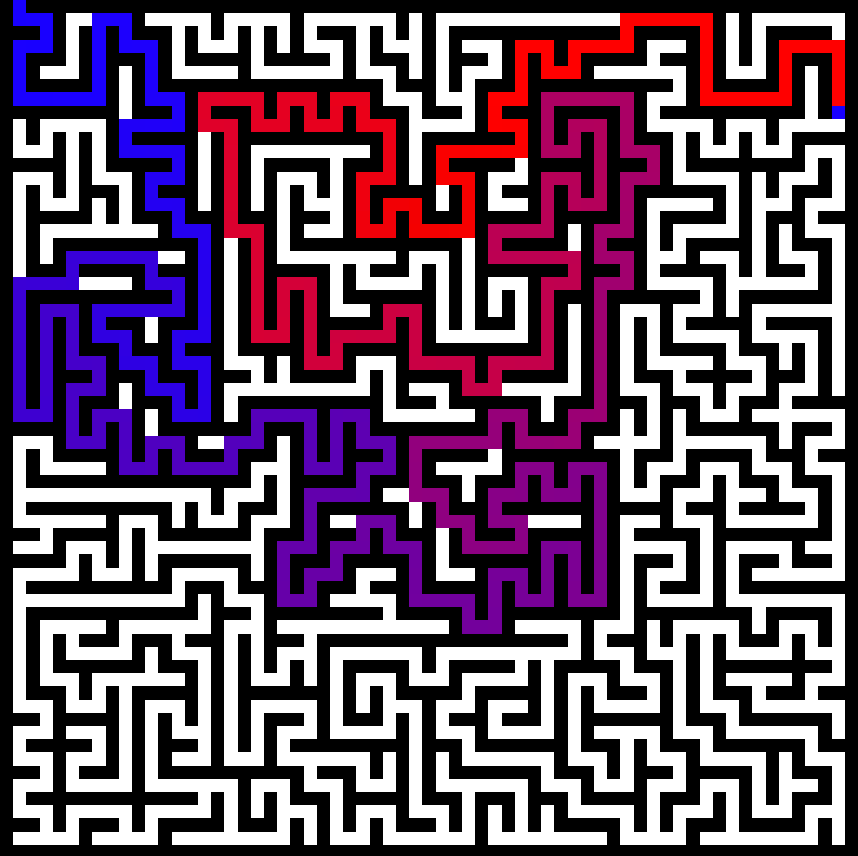
\includegraphics[width=0.8\linewidth]{img/maze_solved}
	\caption{Maze solved}
	 \label{fig:mazesolved}
\end{minipage}

\end{figure}


\section{Experiments}
Using Dijkstra's algorithm the experiments were to measure the running time by changing the size of the maze. The difficulty between the first maze and the last is tripled in fact you can see how (Figure \ref{fig:timedijkstra}), even if the resolution times are very short, there is a difference between the first and the last resolution time. Obviously the red agent is always placed at random so it is difficult to make fair comparisons but it can be noted that the execution time has an increase.

\begin{figure}
\centering
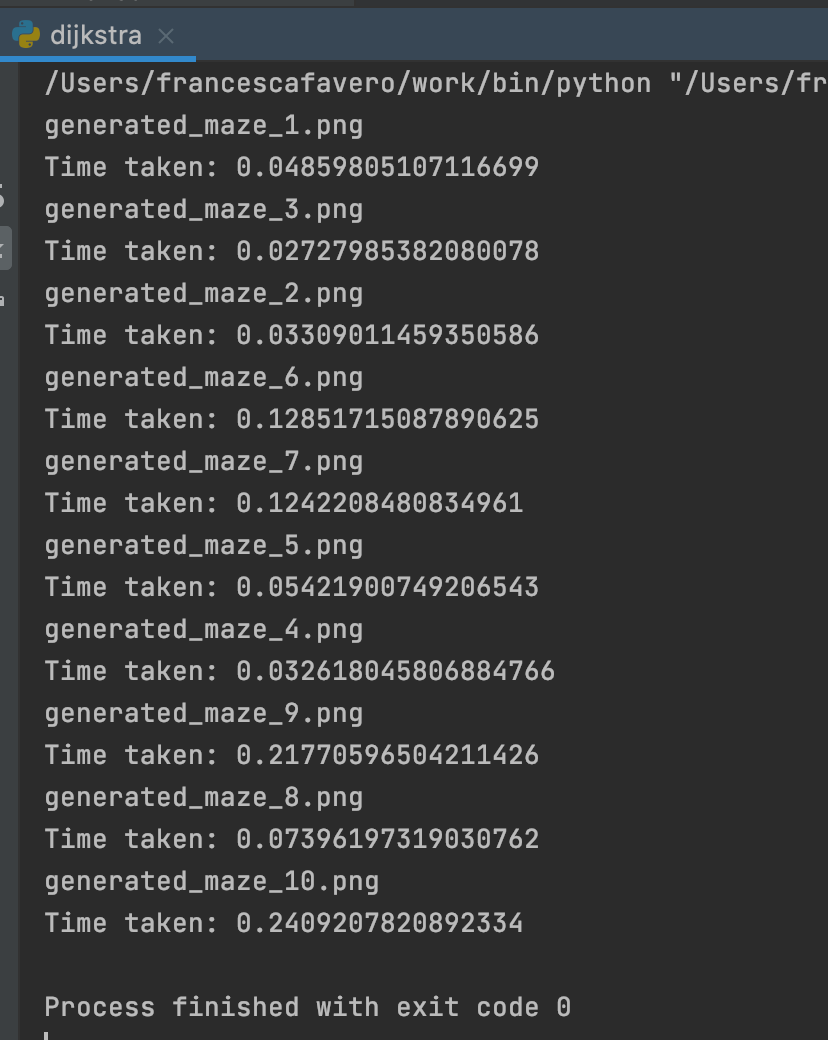
\includegraphics[width=0.7\linewidth]{img/timeDijkstra}
\caption{Time Taken by Dijkstra Algorithm}
\label{fig:timedijkstra}
\end{figure}

